%************************************************
\chapter{HMRF clustering in the brain of \platyfull{}}\label{ch:biology} 
%************************************************
After validating our method using simulated data, we next studied the biological meaning of each of the $K=33$ clusters generated by applying the HMRF model to the real data. To do this, we combined each cluster's spatial location with its corresponding expression parameter $\theta_{h} = (\theta_{h,1},\dots,\theta_{h,m})$. The latter parameter allows a stereotypical expression ``fingerprint" to be associated with every cluster.\\

	\section{Downstream analysis opportunities offered by the model}
		\subsection{Signification of Theta}
		\subsection{Cluster specific gene scoring}
	In practice, not all of the 86 genes will provide insight into the biological function of a given cluster. For instance, in the case of a ubiquitously expressed gene, $g$, the value of $\mathbf{\theta_{.,g}}$ will be high for all clusters. To overcome this problem, we developed a score, $S$, for each gene, $m$ and each cluster $h$, where:
\begin{align*}
s_{hm} = \frac{\theta_{hm}}{\sum_{a} \theta_{am}}.
\end{align*}

For each gene, $m$, and cluster, $h$, $s_{hm}$ is large if gene $m$ is specific to cluster $h$. Consequently, the top scoring 3 or 4 genes for each cluster will represent a specific stereotypical expression pattern that will help us infer or confirm the identity of the functional tissue represented by each cluster.\\

	\section{Choosing K with the BIC on biological data}
	As shown in Figure \ref{fig:realBIC} (blue dots), the BIC does not reach a clear minimum when applied to all cells in the brain but instead reaches a plateau after a given number of clusters. This is most likely due to the highly, but not perfectly symmetrical nature of the brain: with a small $K$, the same ``tissue" on both the left and the right hand side of the brain will belong to the same cluster. However, because the two sides of the brain are not perfectly symmetrical, as $K$ increases the left and right part of the same ``tissue" will be clustered separately. As a result, the likelihood continues to increase sufficiently to explain the flattened BIC curve. Moreover, this hypothesis seems to be confirmed by the fact that when computing the BIC on the right and left side of the brain separately, the curve has in both cases a clear minimum as shown in Figure \ref{fig:realBIC} (red and green dots). Given this, we opted to choose $\hat{K}$ as the point where the BIC curve reaches a plateau.
	
	\begin{figure}[h]
\centerline{\includegraphics[width=0.6\linewidth]{gfx/chapter6/real_BIC.png}}
\caption{{\bf BIC results on biological data.} Results are shown for $K \in [4,80]$ (x axis) with the full brain, and the two left and right half separately. The y axis shows the BIC value in \% of the highest BIC value for each dataset.}
\label{fig:realBIC}
	\end{figure}

	\section{Finding known biological structures to validate the method}
	To provide confidence in our approach, we first considered well characterised regions within the {\it{Platynereis}} brain.
		\subsection{\platy{}'s eyes}
		Arguably the best-studied regions of the brain in {\it{Platynereis}} are the eyes: the brain has 4 eyes, two larval and two adult, and their locations and expression fingerprints are well known. As shown in Figure \ref{fig:valideyesclust}, our approach generates two spatially coherent clusters that correspond to each of these regions. Importantly, the genes that best characterise these clusters are biologically meaningful: {\it{rOpsin}} and {\it{rOpsin3}}, both members of the well-described opsin family of photosensitive molecules \cite{terakita05,randel13}, best distinguish the adult eye and larval eyes respectively, consistent with the in-situ data images shown in Figure \ref{fig:valideyesinsitu}.
		
	\begin{figure}[bth]
        \myfloatalign
        \subfloat[{\bf Eyes in the brain of Platynereis as clustered by the HMRF method.} Adult and larval eyes in separate clusters with their top 3 most representative genes.]
        {\label{fig:valideyesclust}
        \includegraphics[width=.45\linewidth]{gfx/chapter6/eyes.png}} \quad
        \subfloat[{\bf In-situ hybridization image for rOpsin and rOpsin3 in the full brain at 48hpf (Apical view).} Z-projection of the expression of rOpsin (red) in both the adult eyes and the larval eyes, rOpsin3 (green) specifically in the larval eyes and co-expression areas in some areas of the larval eyes in the full brain of {\it{Platynereis}} at 48hpf. The white circle is a schematic outline of the brain.  This image been obtained directly from the data obtained in \cite{Tomer10}]
        {\label{fig:valideyesinsitu}%
         \includegraphics[width=.45\linewidth]{gfx/chapter6/insitu.png}}
        \caption{{\bf Validating the eyes clusters generated by the HRMF clustering.}}
        \label{fig:valideyes}
	\end{figure}
	
	
		\subsection{Mushroom bodies}
		As well as the eyes, a second region of the {\it{Platynereis}} brain, the mushroom bodies (which corresponds to the pallium, layers of neurons that cover the upper surface of the cerebrum in vertebrates \cite{Tomer10}), are also clearly identified by our approach (Figure \ref{fig:validmush}).
		
	\begin{figure}[h]
\centerline{\includegraphics[width=0.6\linewidth]{gfx/chapter6/mush.png}}
\caption{{\bf Mushroom bodies in the brain of Platynereis as clustered by the HMRF method.} Mushroom bodies and their most representative genes.}
\label{fig:validmush}
	\end{figure}
		\subsection{Motor regions}

	\section{Generating functional hypothesis about unknown biological tissues}
	As well as identifying clusters corresponding to known cell types, we also identified clusters that might correspond to less well studied subtypes with specific biological functions. In Figure \ref{fig:eyes_muscles}, the green cluster defines a region on the basal side of the larvae that can be associated both by its localization and by its most representative genes ({\it{MyoD}} \cite{weintraub91,michelson90} and {\it{LDB3}} \cite{krcmery10,marziliano07}) with the starting point of the developing muscles of the adult animal. Indeed, {\it{MyoD}} has been shown to play a key role in the differentiation of muscles during development in vertebrates and invertebrates \cite{weintraub91,michelson90} and {\it{LDB3}} codes for the protein LDB3, which interacts with the myozenin gene family that has been implicated in muscle development in vertebrates \cite{marziliano07}.\\

	\begin{figure}[h]
\centerline{\includegraphics[width=0.6\linewidth]{gfx/chapter6/eyes_muscles.png}}
\caption{{\bf A putative tissue of developing neurons between the eyes and the larvae's developing muscles.} The yellow and red clusters are the eyes as seen on figure \ref{fig:valid}. The green cluster represents the developing muscles on the basal side of the larvae, as the location and the most specific genes strongly suggest. The pink cluster is a putative tissue that makes an interesting link between the eyes and the muscles. The most representative gene of this tissue is Phox2, a homeodomain protein required for the generation of visceral motor-neurons in \emph{Drosophila} \cite{briscoe99}}
\label{fig:eyes_muscles}
	\end{figure}

	Given the location of the eyes and the developing muscles, the location of the pink cluster in Figure \ref{fig:eyes_muscles} is interesting. This cluster surrounds the larval eyes, the adult eyes and reaches the hypothetically developing muscles described above. Looking at the most representative genes for this pink cluster, it is interesting to note the presence of {\it{Phox2}}, a homeodomain protein that has been shown to be necessary for the generation of visceral motor-neurons (neurons of the central nervous system that project their axons to directly or indirectly control muscles) as described generally in \cite{brunet02} and in \emph{Drosophila} \cite{briscoe99}. The second most representative gene, {\it{COE}}, has also been shown to play a role in \emph{Platynereis} and \emph{Drosophila} neural tissue development \cite{demilly11}. In this context, although we lack biological validation, we can hypothesise that the cells within this particular cluster could be developing neurons that link the eyes to the muscles of \emph{Platynereis}. Although this hypothesis remains purely speculative and would need validation in the laboratory, we believe this example is an interesting proof-of-concept that our clustering method can prove useful for hypothesis generation. Indeed, the analysis of the parameter values and the spatial localization attached to the clusters has allowed us to place with a reasonable level of confidence a functional hypothesis about a tissue that was not clearly defined either spatially or functionally. It is also interesting to note that hClust does not separate either putative region when clustering the same data with the same number of clusters. \\

	\section{Discussion}
		\subsection{Validity of the model's independence hypothesis}
		In our model we assume that, conditional upon the allocation of a cell to a cluster, the gene expression levels can be described by independent Bernoulli distributions. This is a reasonable assumption in the context of the 86 genes chosen by Tomer et al. \cite{Tomer10}, since they were selected to have largely orthogonal expression profiles. In other words, they were chosen since they were known to correspond to distinct and potentially interesting regions of the {\it{Platynereis}} brain. However, in many other settings a larger number of genes, many with correlated expression profiles (i.e., genes in the same regulatory network) will be profiled and this assumption will be invalid. Consequently, extending the model to allow for dependence structure in the emission distributions will be a critical challenge.
		\subsection{Shortcomings of the method}
		talk about the fact that hypothesis need to be validated. Also K is not necessarly the true number of cluster depending on the number of genes considered. Also quantitative data with poisson distibution to open on the conclusions
	



%*****************************************
%*****************************************
%*****************************************
%*****************************************
%*****************************************
